%%
%% This is file `tikzposter-template.tex',
%% generated with the docstrip utility.
%%
%% The original source files were:
%%
%% tikzposter.dtx  (with options: `tikzposter-template.tex')
%%
%% This is a generated file.
%%
%% Copyright (C) 2014 by Pascal Richter, Elena Botoeva, Richard Barnard, and Dirk Surmann
%%
%% This file may be distributed and/or modified under the
%% conditions of the LaTeX Project Public License, either
%% version 2.0 of this license or (at your option) any later
%% version. The latest version of this license is in:
%%
%% http://www.latex-project.org/lppl.txt
%%
%% and version 2.0 or later is part of all distributions of
%% LaTeX version 2013/12/01 or later.
%%


\documentclass{tikzposter} %Options for format can be included here

\usepackage{todonotes}

\usepackage[tikz]{bclogo}
\usepackage{lipsum}
\usepackage{amsmath}

\usepackage{booktabs}
\usepackage{longtable}
\usepackage[absolute]{textpos}
\usepackage[it]{subfigure}
\usepackage{graphicx}
\usepackage{cmbright}
%\usepackage[default]{cantarell}
%\usepackage{avant}
%\usepackage[math]{iwona}
\usepackage[math]{kurier}
\usepackage[T1]{fontenc}


%% add your packages here
\usepackage{hyperref}
% for random text
\usepackage{lipsum}
\usepackage[english]{babel}
\usepackage[pangram]{blindtext}

\colorlet{backgroundcolor}{blue!10}

 % Title, Author, Institute
\title{Group Outlying Aspects Mining}
\author{Jincai Ma}
\institute{ Xi'an Shiyou University, China \\
}
%\titlegraphic{logos/tulip-logo.eps}

%Choose Layout
\usetheme{Wave}

%\definebackgroundstyle{samplebackgroundstyle}{
%\draw[inner sep=0pt, line width=0pt, color=red, fill=backgroundcolor!30!black]
%(bottomleft) rectangle (topright);
%}
%
%\colorlet{backgroundcolor}{blue!10}

\begin{document}


\colorlet{blocktitlebgcolor}{blue!23}

 % Title block with title, author, logo, etc.
\maketitle

\begin{columns}
 % FIRST column
\column{0.5}% Width set relative to text width

%%%%%%%%%% -------------------------------------------------------------------- %%%%%%%%%%
 %\block{Main Objectives}{
%  	      	\begin{enumerate}
%  	      	\item Formalise research problem by extending \emph{outlying aspects mining}
%  	      	\item Proposed \emph{GOAM} algorithm is to solve research problem
%  	      	\item Utilise pruning strategies to reduce time complexity
%  	      	\end{enumerate}
%%  	      \end{minipage}
%}
%%%%%%%%%% -------------------------------------------------------------------- %%%%%%%%%%


%%%%%%%%%% -------------------------------------------------------------------- %%%%%%%%%%
\block{Introduction}{
  
  	
    \begin{description}
      
  	\item[The Data Source] The data comes from Kaggle https://www.kaggle.com/c/bike-sharing-demand
  	
  	\item[Project Purpose] Use recipe ingredients to categorize the cuisine.\\
      Given the name of the condiment, predict the cuisine to which the dish belongs.
  	\end{description}

  	
}
%%%%%%%%%% -------------------------------------------------------------------- %%%%%%%%%%


%%%%%%%%%% -------------------------------------------------------------------- %%%%%%%%%%
\block{Related Field Name Interpretation}{

\begin{itemize}
    \item
    In the dataset,  including the recipe ID, the dish, and the list of ingredients for each recipe (variable length).The data is stored in JSON format. \\
    1.train.json- A training set that contains the recipe ID, dish type, and ingredient list\\
    2.test.json- A test set containing a recipe ID and a list of ingredients\\
    3.sample\_submission.csv- Properly formatted sample submission document
\end{itemize}


}
%%%%%%%%%% -------------------------------------------------------------------- %%%%%%%%%%

%%%%%%%%%% -------------------------------------------------------------------- %%%%%%%%%%
\block{ Data Import And Introduction}{
                                       
    \begin{itemize}
        \item
        Import the JSON file with Pandas:
        We can get the data set of dish names, including 39774 training data and 9944 test samples.
        \item To see the distribution of our data set and the total variety of dishes, we printed out some of the data samples.
    \end{itemize}
    \begin{minipage}{1\linewidth}
        \centering
        \includegraphics[width=1\textwidth]{pic1/1.png} 
    \end{minipage}

    \begin{itemize}
        \item
        Total dish classification\\
        There are 20 dishes in total, which are:
        ['brazilian' 'british' 'cajun\_creole' 'chinese' 'filipino' 'french'
         'greek' 'indian' 'irish' 'italian' 'jamaican' 'japanese' 'korean'
         'mexican' 'moroccan' 'russian' 'southern\_us' 'spanish' 'thai'
         'vietnamese']
        
    \end{itemize}
    
}
%%%%%%%%%% -------------------------------------------------------------------- %%%%%%%%%%
\block{Data Analysis}{
    
    \begin{itemize}                            
        \item The data set is divided into Features and Target Variables.
        \item Features:'ingredients', we were given the names of the ingredients contained in each dish.
        Target variable:'cuisine', is the classification of cuisines that we want to predict.
        \item Extract the Feature of training data set into train\_integredients variable,extract the Target Variables into the train\_Targets variable
    \end{itemize}
    \begin{minipage}{0.7\linewidth}
        \centering
        \includegraphics[width=0.7\textwidth]{pic1/2.png} 
    \end{minipage}
   
   
}

% SECOND column
\column{0.5}
 %Second column with first block's top edge aligned with with previous column's top.

%%%%%%%%%% -------------------------------------------------------------------- %%%%%%%%%%
\block{Data Analysis}{
    
    \begin{itemize}                            
        \item
        What are the top 10 most frequently used ingredients?
        \item What are the 10 most common ingredients in filipino,greek and Italian cuisine?
    \end{itemize}
    \begin{minipage}{0.5\linewidth}
        \centering
        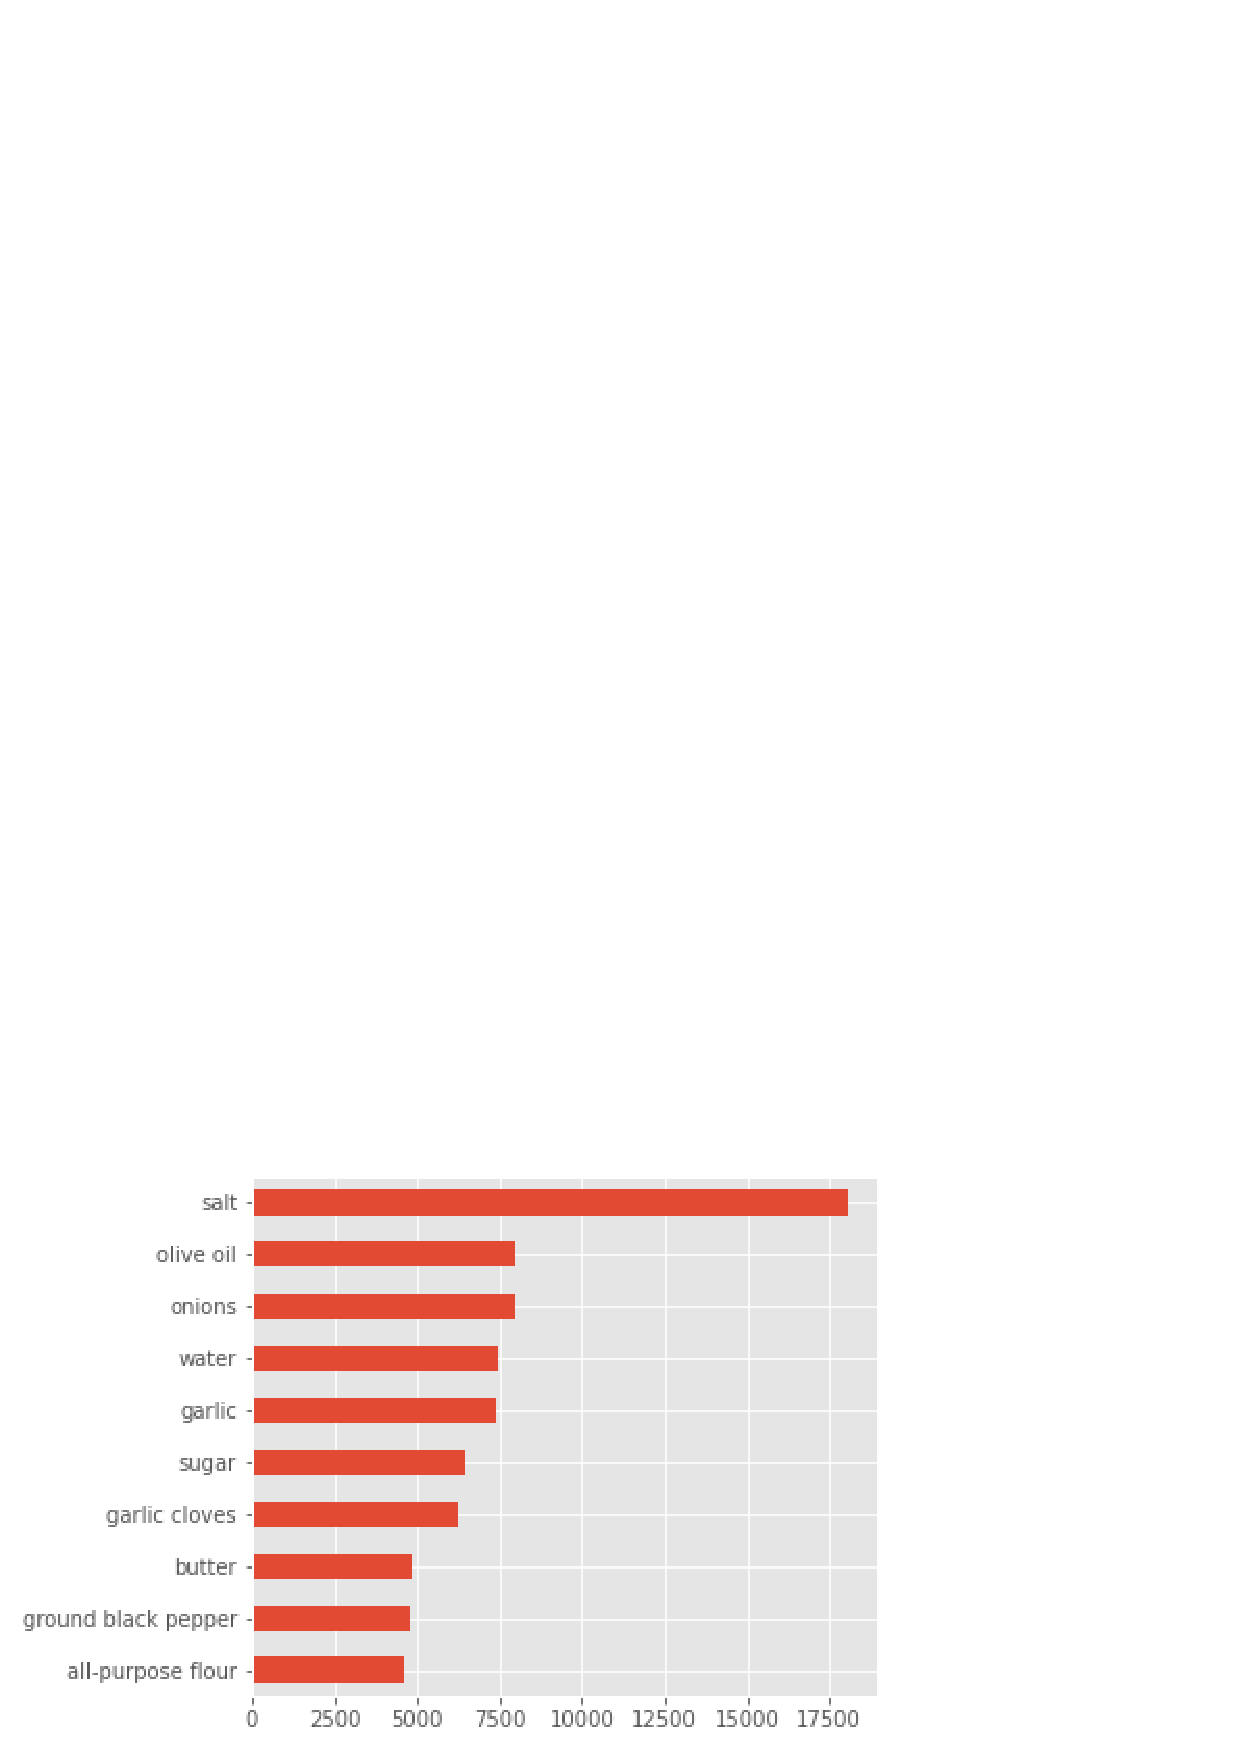
\includegraphics[width=0.6\textwidth]{pic1/cooking.png} 
    \end{minipage}
    \begin{minipage}{0.5\linewidth}
        \centering
        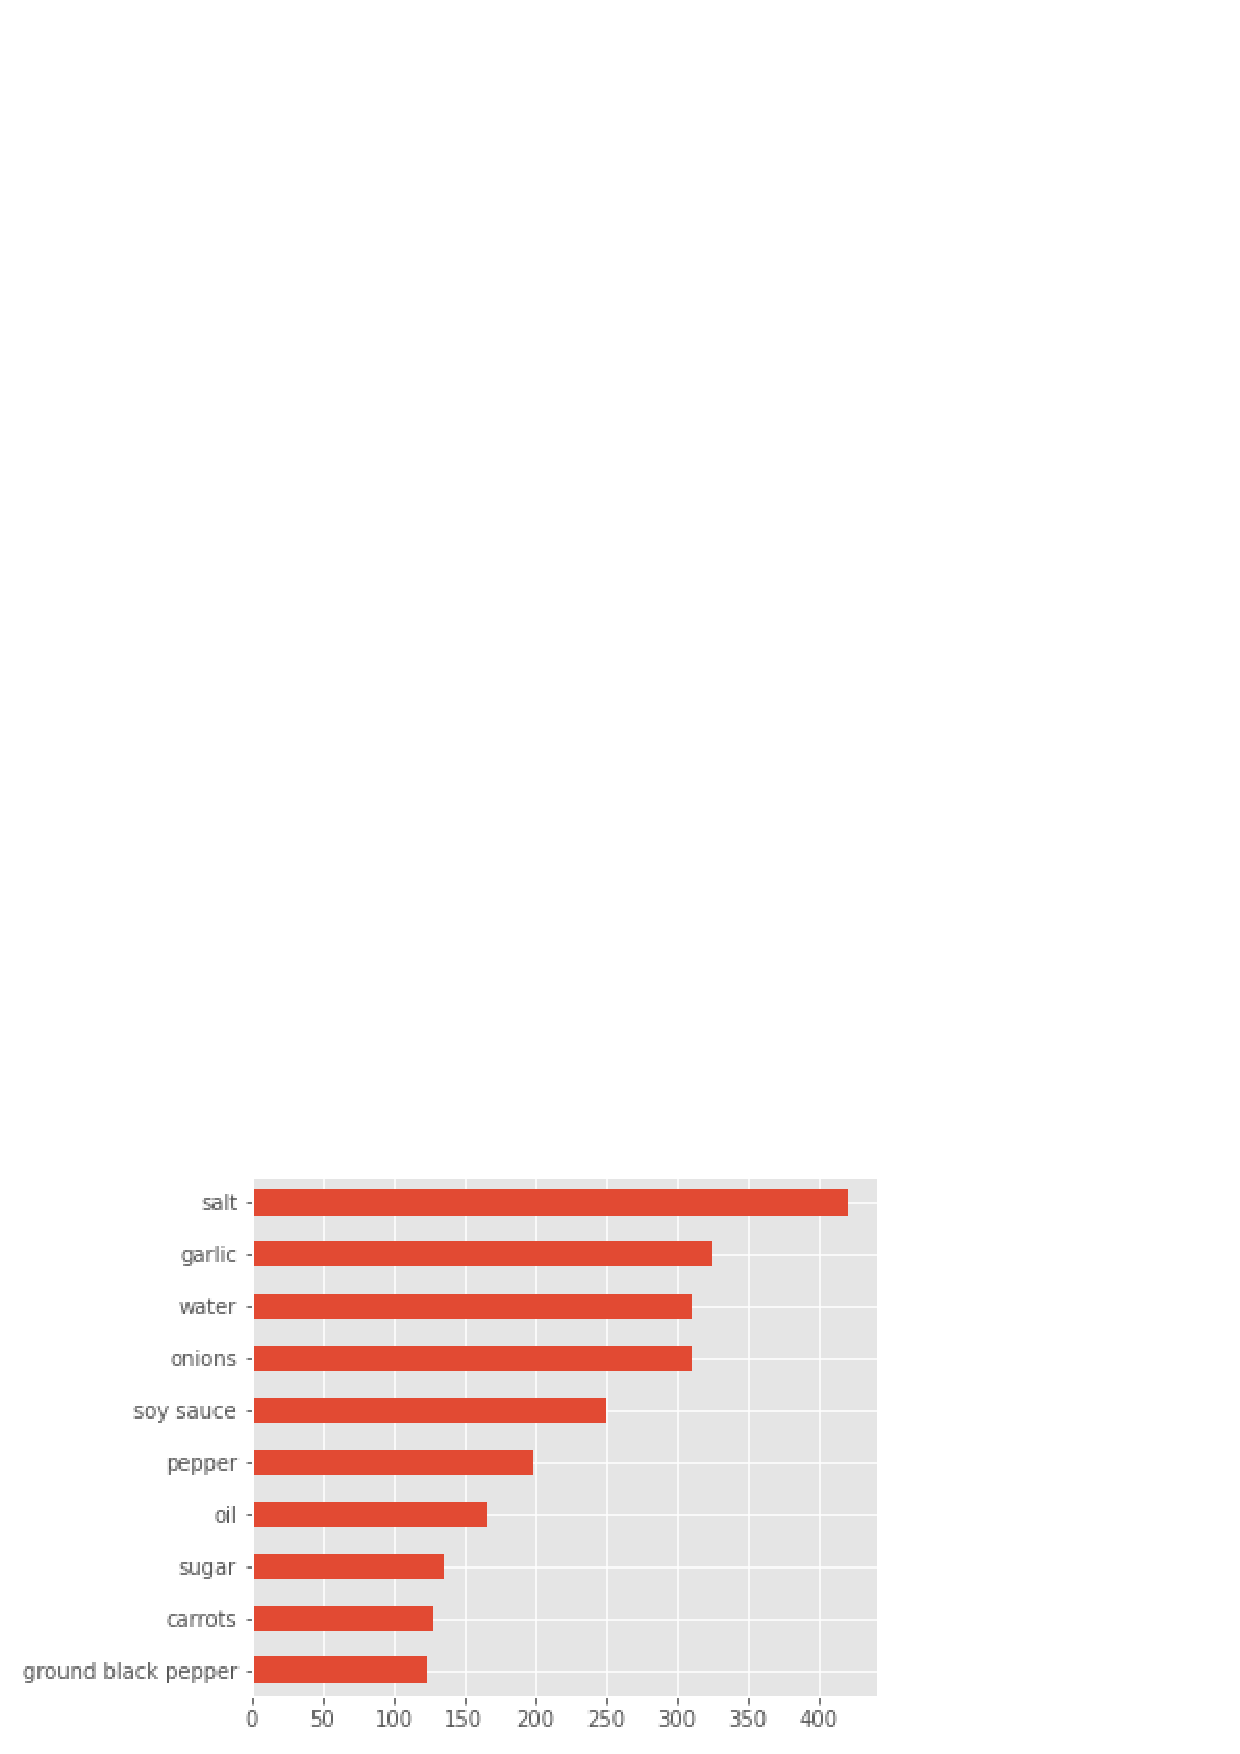
\includegraphics[width=0.6\textwidth]{pic1/filipino.png} 
    \end{minipage}
    \begin{minipage}{0.5\linewidth}
        \centering
        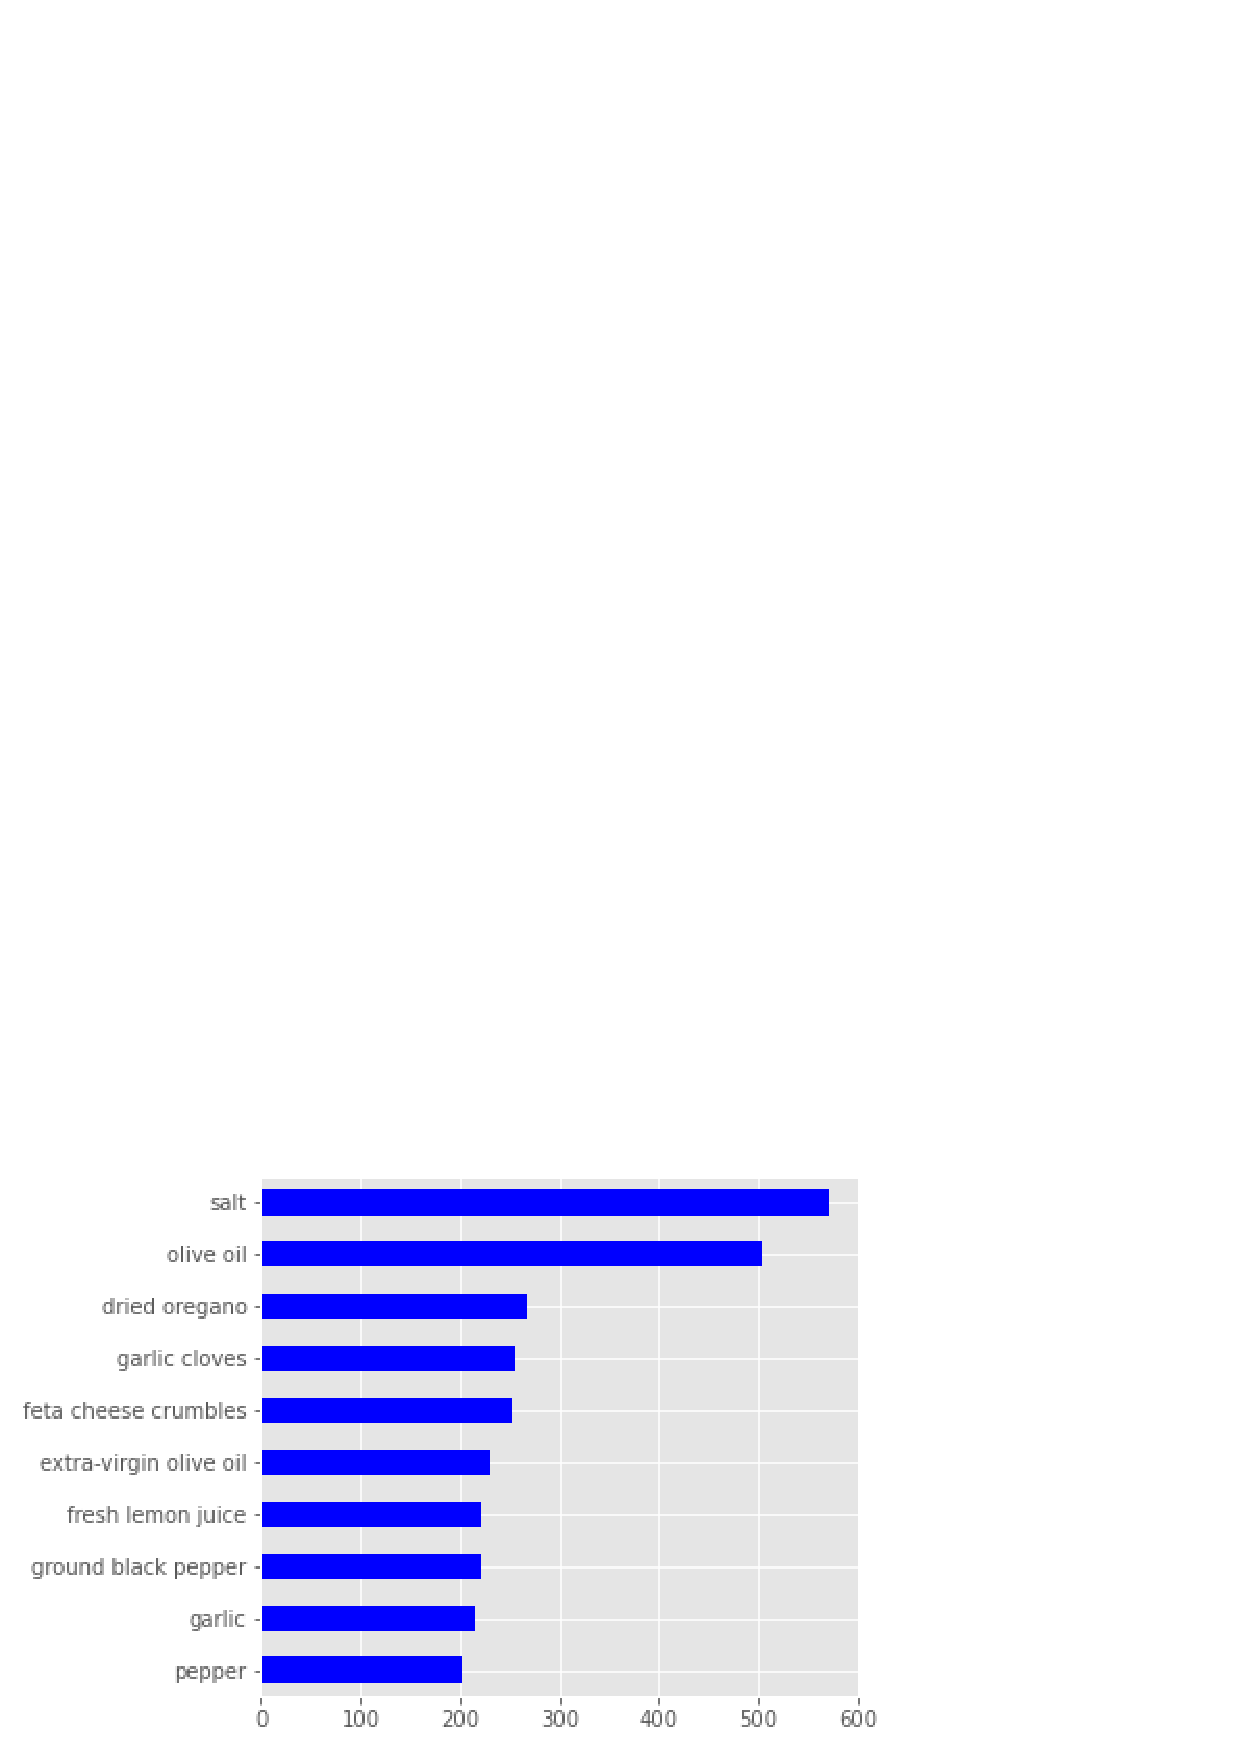
\includegraphics[width=0.6\textwidth]{pic1/greek.png} 
    \end{minipage}
    \begin{minipage}{0.5\linewidth}
        \centering
        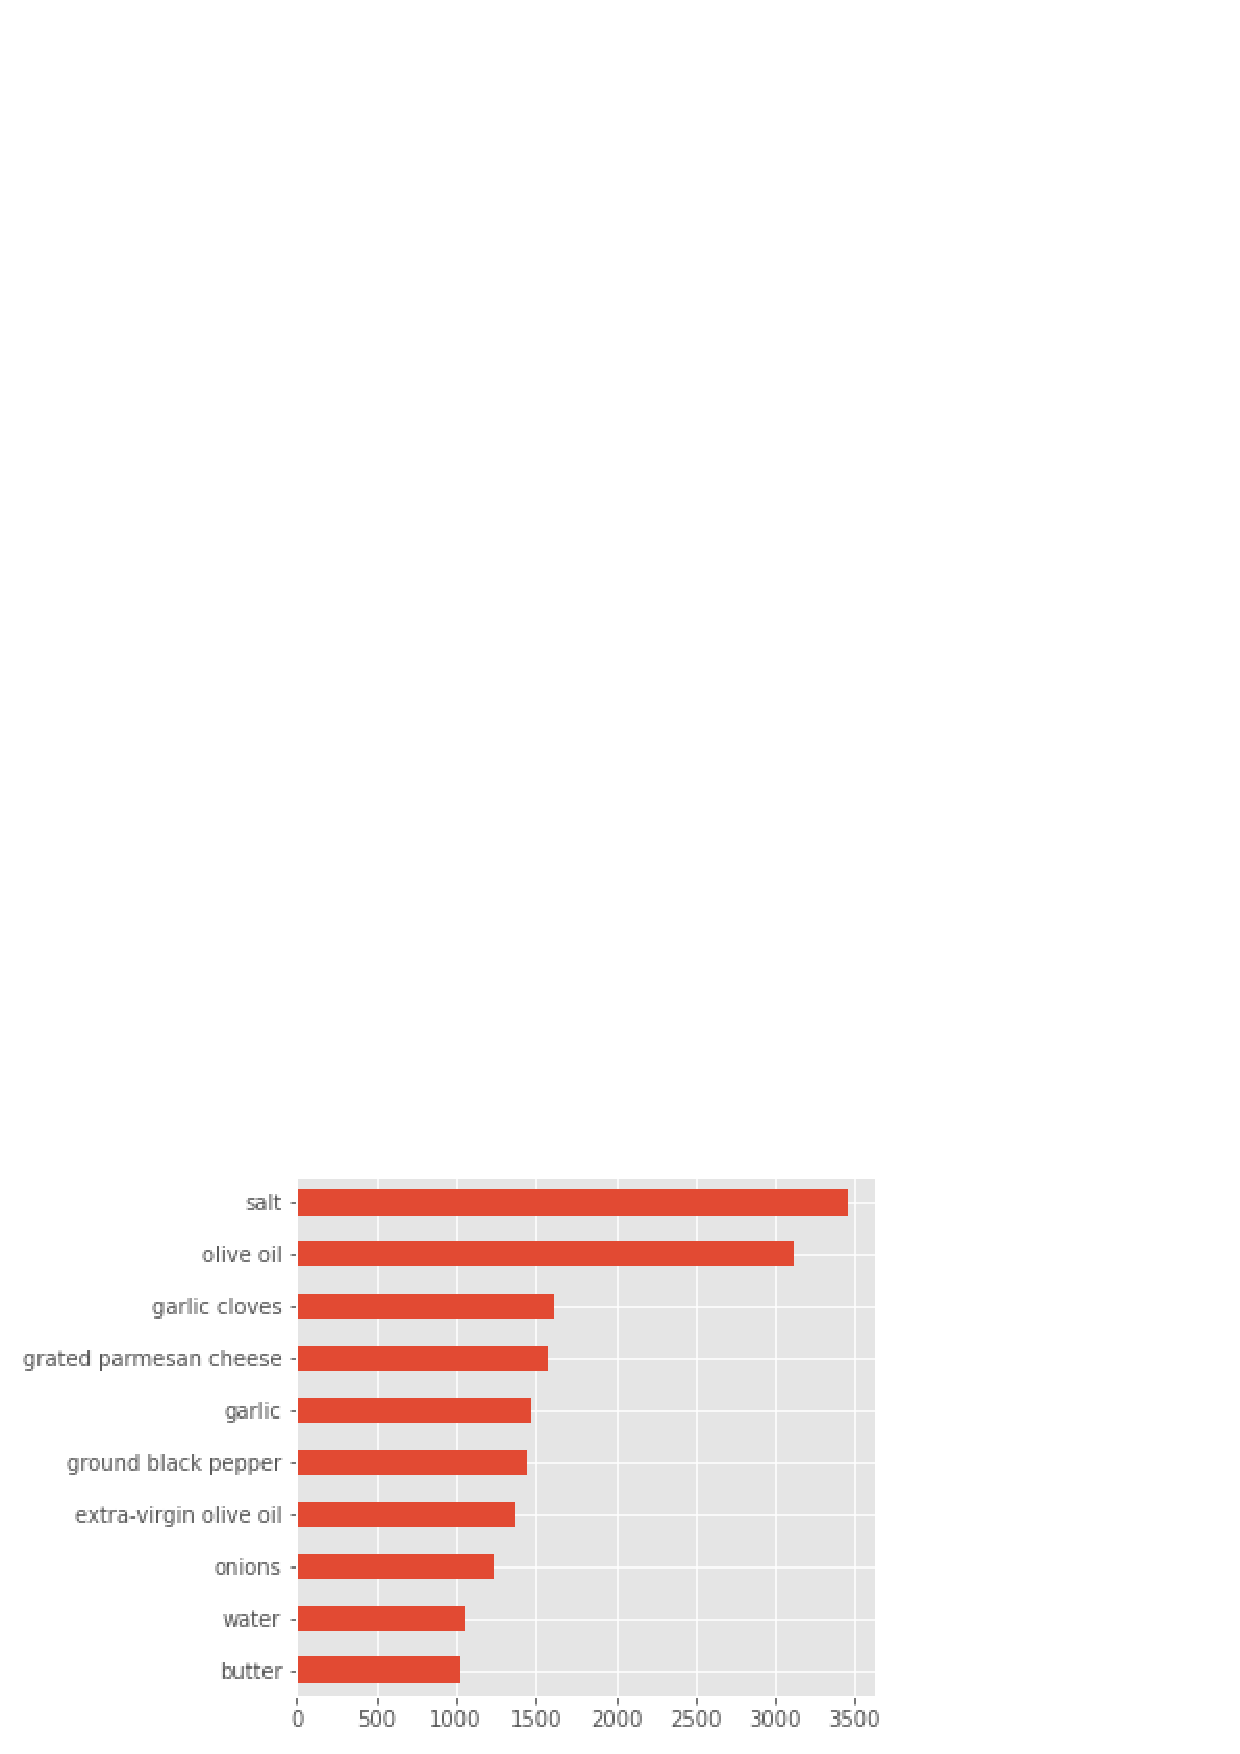
\includegraphics[width=0.6\textwidth]{pic1/italian.png} 
    \end{minipage}
   
}
%%%%%%%%%% -------------------------------------------------------------------- %%%%%%%%%%
% Second column - first block
\block{Data cleaning}{
   
    \begin{itemize}                            
        \item
        Since dishes contain a large number of ingredients, and since the same ingredients can vary in numbers, tenses, and so on, we considered sifting through a potatos to remove any such differences
    \end{itemize}
    \begin{minipage}{1\linewidth}
        \centering
        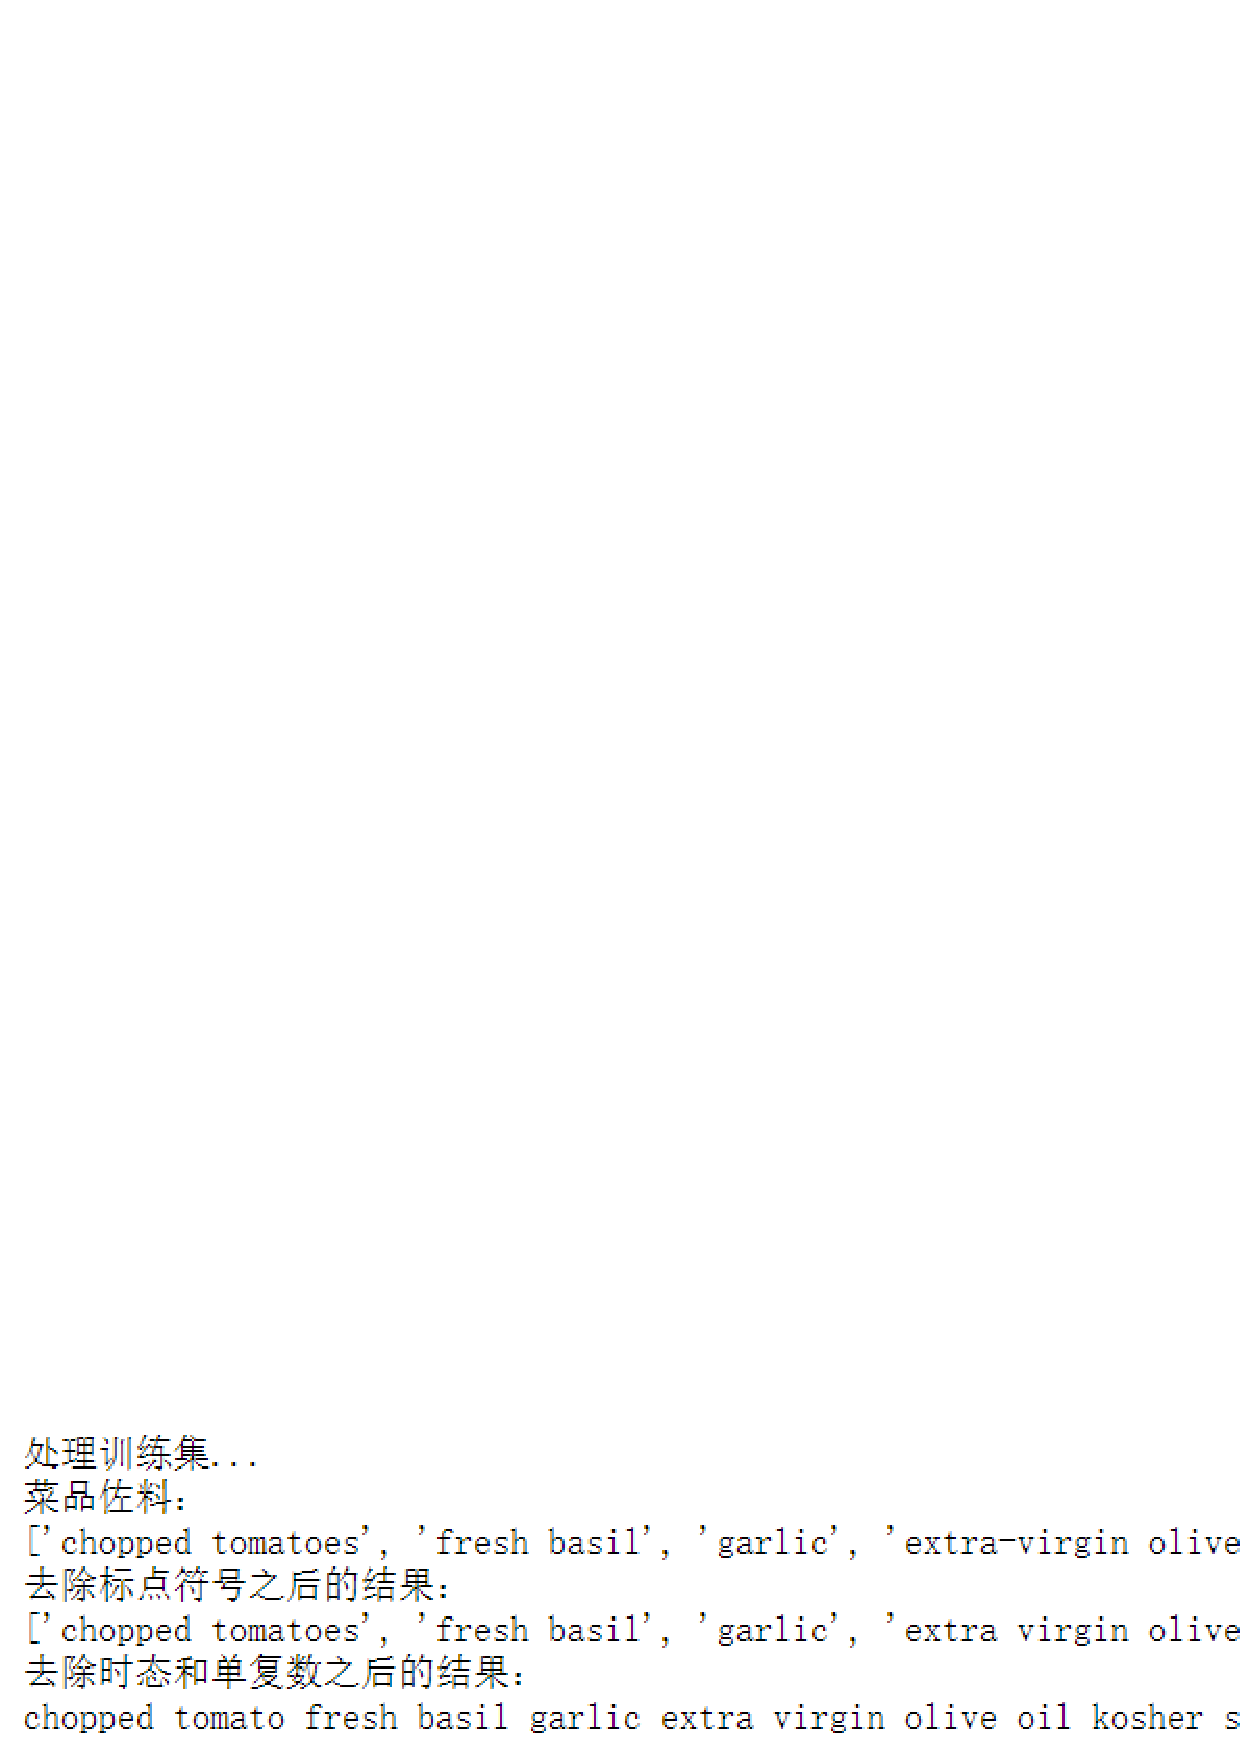
\includegraphics[width=0.8\textwidth]{pic1/clean1.png} 
    \end{minipage}
    \begin{minipage}{1\linewidth}
        \centering
        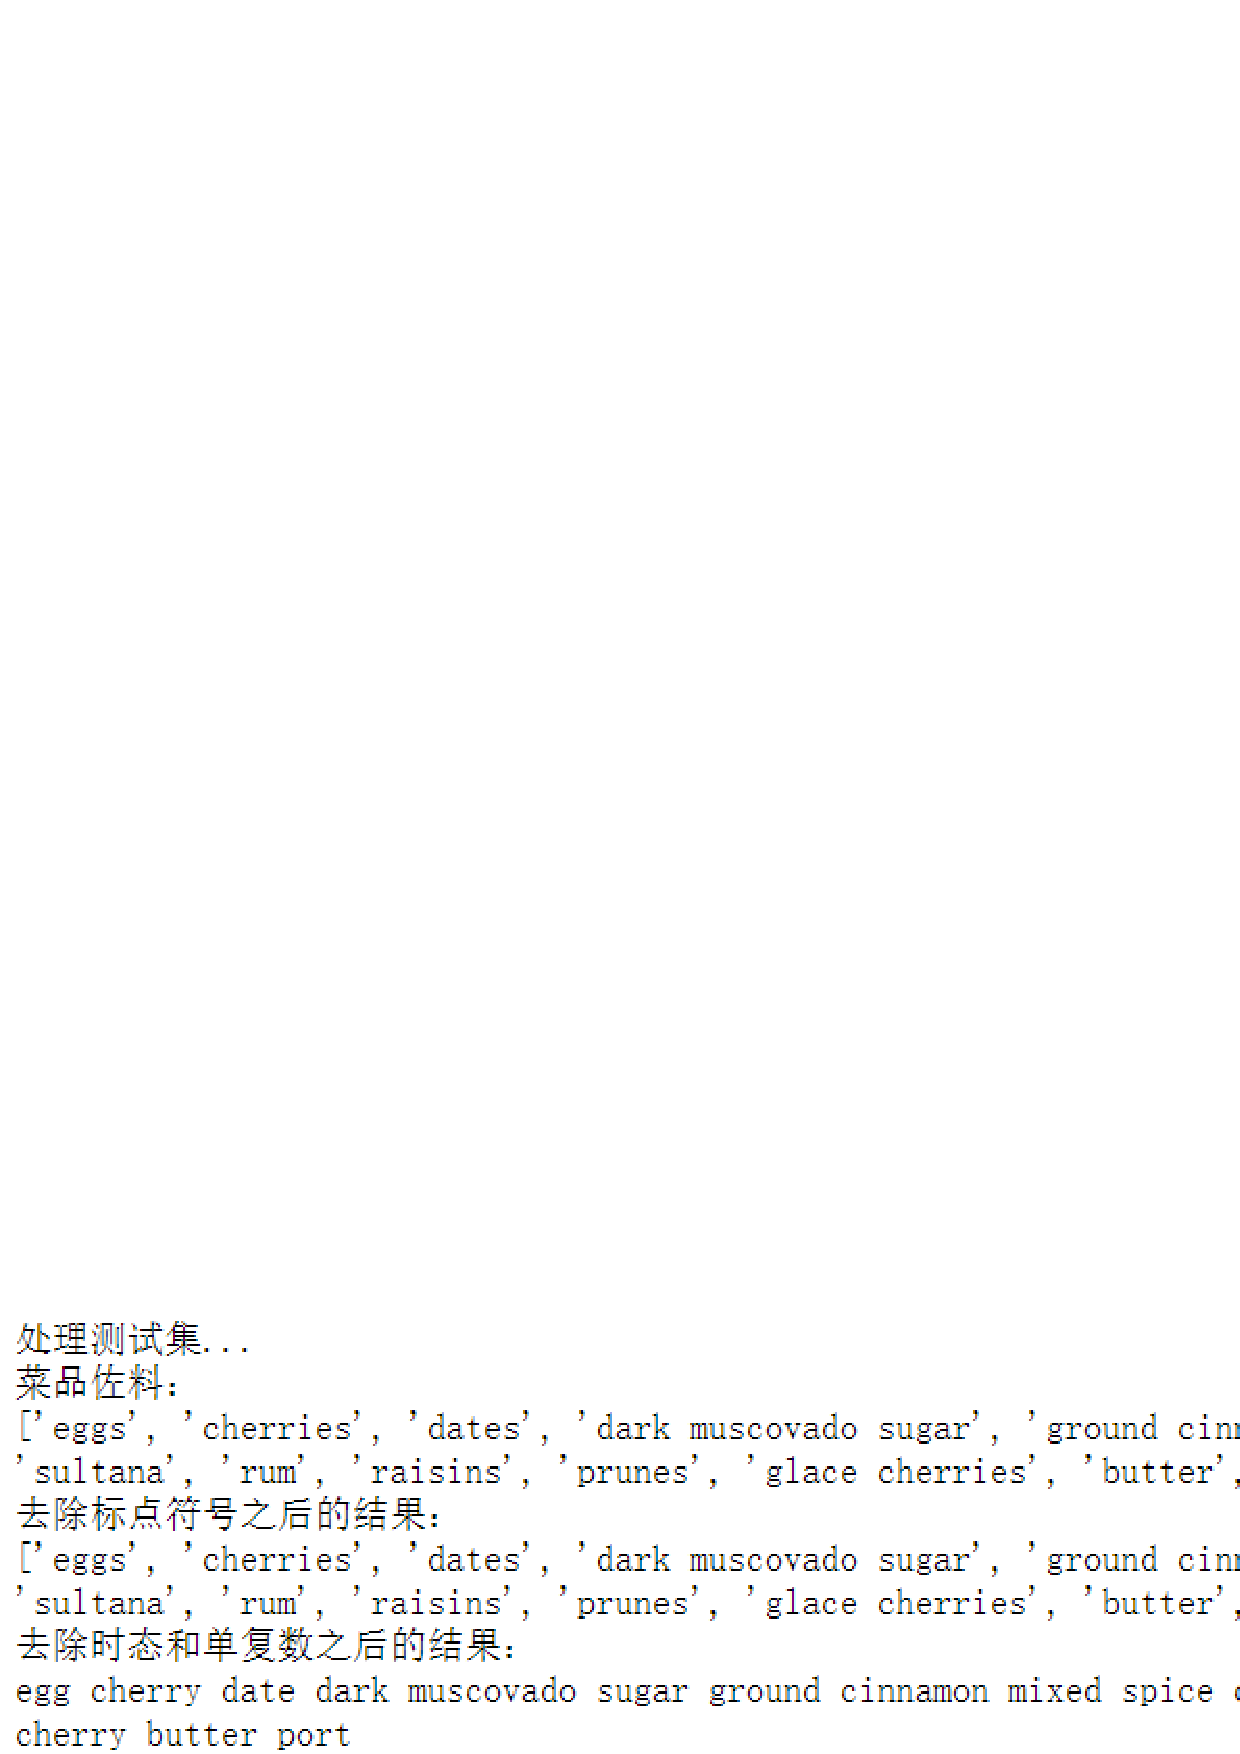
\includegraphics[width=0.8\textwidth]{pic1/clean2.png} 
    \end{minipage}
}

%%%%%%%%%% -------------------------------------------------------------------- %%%%%%%%%%
\block{Feature extraction}{
   
    \begin{itemize}                            
        \item We convert the ingredients of the dish into a numerical feature vector.Consider that most dishes include salt, water, sugar, butter, etc,We will consider weighting the seasonings according to the occurrence times of the seasonings, that is, the more the occurrence times of the condiments, the lower the discriminability of the condiments.The feature we adopt is TF-IDF.
        \item We can get the characteristics:\lbrack'greek','southern\_us','filipino','indian','indian',\\
        'jamaican','spanish','italian','mexican','italian'\rbrack
    \end{itemize}
    
}

%%%%%%%%%% -------------------------------------------------------------------- %%%%%%%%%%
\block{Build Model}{

\begin{description}
    \item[]
    1.Separate the training set and test set.\\
    2.Remove unwanted eigenvalues:'casual','count','datetime','registered','date','atemp','month','year','season','weather'\\
    3.Cross validation is used to determine the optimal parameters.\\
    4.View the selected optimal parameters:{max depth: 20, n estimators: 150}\\
    5.Apply the optimal parameters to the model, it can be obtained\\
    Accuracy on test set : 0.6945996275605214
\end{description}


}
%%%%%%%%%% -------------------------------------------------------------------- %%%%%%%%%%


% Second column - second block
%%%%%%%%%% -------------------------------------------------------------------- %%%%%%%%%%
\block[titlewidthscale=1, bodywidthscale=1]
{Conclusion}
{
\begin{description}
  \item[]
  Through this Kaggle project, I practiced by myself to have a deeper understanding of data visualization and to explore the structure and rules of data by means of drawing and tabulating.

\end{description}
}
%%%%%%%%%% -------------------------------------------------------------------- %%%%%%%%%%


% Bottomblock
%%%%%%%%%% -------------------------------------------------------------------- %%%%%%%%%%
\colorlet{notebgcolor}{blue!20}
\colorlet{notefrcolor}{blue!20}
\note[targetoffsetx=8cm, targetoffsety=-4cm, angle=30, rotate=15,
radius=2cm, width=.26\textwidth]{
Acknowledgement
\begin{itemize}
    \item
    International Cooperation Project (Y7Z0511101)
    of IIE,
    Chinese Academy of Sciences
 \end{itemize}
}

%\note[targetoffsetx=8cm, targetoffsety=-10cm,rotate=0,angle=180,radius=8cm,width=.46\textwidth,innersep=.1cm]{
%Acknowledgement
%}

%\block[titlewidthscale=0.9, bodywidthscale=0.9]
%{Acknowledgement}{
%}
%%%%%%%%%% -------------------------------------------------------------------- %%%%%%%%%%

\end{columns}


%%%%%%%%%% -------------------------------------------------------------------- %%%%%%%%%%
%[titleleft, titleoffsetx=2em, titleoffsety=1em, bodyoffsetx=2em,%
%roundedcorners=10, linewidth=0mm, titlewidthscale=0.7,%
%bodywidthscale=0.9, titlecenter]

%\colorlet{noteframecolor}{blue!20}
\colorlet{notebgcolor}{blue!20}
\colorlet{notefrcolor}{blue!20}
\note[targetoffsetx=-13cm, targetoffsety=-18cm,rotate=0,angle=180,radius=8cm,width=.96\textwidth,innersep=.4cm]
{
\begin{minipage}{0.3\linewidth}
\centering
\includegraphics[width=24cm]{logos/tulip-wordmark.eps}
\end{minipage}
\begin{minipage}{0.7\linewidth}
{ \centering
 The $11^{th}$ International Conference on Knowledge Science,
  Engineering and Management (KSEM 2018),
  17-16/20/2020,Xi'an, China
}
\end{minipage}
}
%%%%%%%%%% -------------------------------------------------------------------- %%%%%%%%%%


\end{document}

%\endinput
%%
%% End of file `tikzposter-template.tex'.
